\section{Integrals}
\subsection{Gaussian integrals}
A useful integral is the Gaussian integral,
\begin{equation}
    \int_\R \dd z \, \exp(- \frac{1}{2} a z^2) = \sqrt{\frac{2 \pi}{a}},
\end{equation}
for $a \in \R$. The imaginary version,
\begin{equation}
    \int_R \dd z \, \exp(i \frac{1}{2} a z^2 )
\end{equation}
does not converge. However, if we change $a \rightarrow a + i\epsilon$, 
% contour of integration slightly, by rotating it clockwise to $C = \R(1 + i\epsilon)$,
% \begin{figure}
%     \begin{subfigure}{0.4\textwidth}
%         \begin{tikzpicture}
%             \draw (-2, 0) -- (2, 0) node[right] {$\mathrm{Re}(x)$};
%             \draw (0, -2) -- (0, 2) node[above] {$\mathrm{Im}(x)$};
%             \draw[->, thick] (-1.8, 0) -- (1.8, 0);
%         \end{tikzpicture}    
%     \end{subfigure}
%     \begin{subfigure}{0.18\textwidth}
%         \begin{tikzpicture}
%             \draw[->] (-1, 0) -- (1, 0);
%         \end{tikzpicture}
%     \end{subfigure}
%     \begin{subfigure}{0.4\textwidth}
%         \begin{tikzpicture}
%             \draw (-2, 0) -- (2, 0) node[right] {$\mathrm{Re}(x)$};
%             \draw (0, -2) -- (0, 2) node[above] {$\mathrm{Im}(x)$};
%             \draw[->, thick] (-1.8, -0.1) -- (1.8, 0.1);
%         \end{tikzpicture}    
%     \end{subfigure}
% \end{figure}
then the integrand is exponentially supressed.
\begin{equation}
    f(x) = \exp(i \frac{1}{2}a x^2) \rightarrow
    \exp(i\frac{1}{2}a x^2 - \frac{1}{2} \epsilon  x^2),
    % \exp(i \frac{1}{2}a z(t)^2) = \exp(i\frac{1}{2}a t^2(1 + i \epsilon)^2) \sim \exp(-\frac{1}{2}a \epsilon t^2 + i \frac{1}{2}at^2).
\end{equation}
As the integrand falls of exponentially for $x\rightarrow \infty$, and contains no poles in the upper right nor lower left quarter of the complex plane, we may perform a wick rotation by closing the contour as shown in \autoref{Wick rotation}.
\begin{figure}
    \centering
    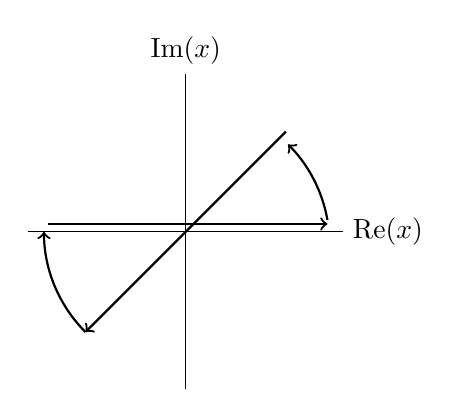
\begin{tikzpicture}
        \draw (-2, 0) -- (2, 0) node[right] {$\mathrm{Re}(x)$};
        \draw (0, -2) -- (0, 2) node[above] {$\mathrm{Im}(x)$};
        \draw[->, thick] (-1.75, 0.1) -- (1.8, 0.1);
        \draw[->, thick] (1.8, 0.15) arc (10:45:1.8);
        \draw[->, thick] ({1.8/sqrt(2)}, {1.8/sqrt(2)}) -- ({-1.8/sqrt(2)}, {-1.8/sqrt(2)});
        \draw[->, thick] ({-1.8/sqrt(2)}, {-1.8/sqrt(2)}) arc (225:180:1.8);
    \end{tikzpicture}
    \caption{Wick rotation}
    \label{Wick rotation}
\end{figure}
This gives the result
\begin{equation}
    \label{complex gauss 1D}
    \int_\R \dd x \, \exp(i \frac{1}{2}(a + i\epsilon) x^2) 
    = \int_{\sqrt{i}\R} \dd x \, \exp(i\frac{1}{2} ax^2)
    = \sqrt{i} \int_\R \dd y\, \exp(-\frac{1}{2} a y^2) = \sqrt{\frac{2 \pi i}{a}}
\end{equation}
where we have made the change of variable $y = (1+i)/\sqrt{2} x = \sqrt{i} x$.

In $n$ dimensions, the Gaussian integral formula generalizes to
\begin{equation}
    I_n = \int_{\R^n} \dd^n x \, \exp{-\frac{1}{2} x_n A_{nm} x_m } =\sqrt{\frac{(2 \pi)^n}{\det(A)}},
\end{equation}
where $A$ is a matrix with $n$ real, positive eigenvalues.
We may also generalize \autoref{complex gauss 1D},
\begin{equation}
    I'_n = 
    \int_{\R^n} \dd^n x \, \exp{i\frac{1}{2} x_n( A_{nm} + i \epsilon \delta_{nm}) x_m } =\sqrt{\frac{(2 \pi i )^n}{\det(A)}}.
\end{equation}

The final generalization is to functional integrals.
The bilinear becomes
\begin{equation}
    x_n A_{nm} x_m \rightarrow \int \dd x \, \varphi(x) A \varphi(x),
\end{equation}
where $A$ is some operator.
The first Gaussian integral becomes
\begin{equation}
    I_\infty = \int \D \varphi \, \exp(- \frac{1}{2} \int \dd x \, \varphi(x) A \varphi(x) )
    = C (\det(A))^{-1/2}.
\end{equation}
$C$ is here a divergent constant, but will either fall away as we are only looking at the logarithm of $I_\infty$ and are able to throw away additive constants, or ratios between quantities which are both multiplied by $C$.


